\section{Basic Properties}
\label{sec:basic}

After collecting data, we first conducted a set of analysis 
to learn various basic properties of submission files, 
submission sources, and anti-virus engines.
These properties give an overview of how real-world submissions and anti-virus engines are like
and serve as the foundation for our more advanced analysis in the next two sections. 





%\noindent{\textit{\underline{Submission temporal, geo-location, and size distribution.}}}

\subsection{Submission Temporal, Geo-location, and Size Distribution}
\label{sec:basicanal}


\begin{figure}[t!]
\begin{center}
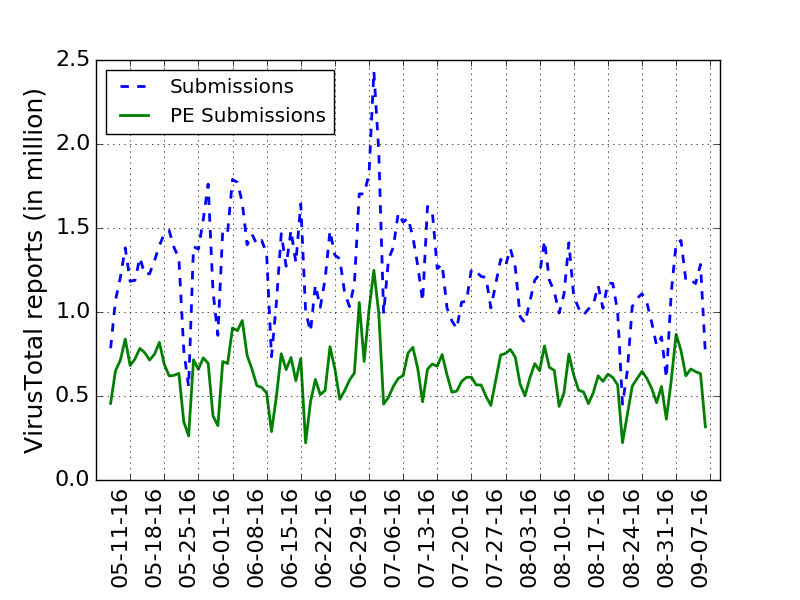
\includegraphics[width=2in]{figure/Submissions}
\caption{The number of files and PE files.
%{\footnotesize{
(The number of suspicious files and the number of PE files submitted to VirusTotal from 05/07/2016 to 09/06/2016.)
%}
}
\label{fig:subnum}
\end{center}
%\vspace{-0.25in}
\end{figure}


Figure~\ref{fig:subnum} plots the number of submissions of all types and the number of \pe\ submissions per day 
over the whole collection period.
There are a large amount of submissions every day
and the amount of submissions is fairly stable over the whole collection period.
The same conclusion can be made to \pe\ submissions.

One PE file could be submitted more than once to VirusTotal. 
On average, each PE file was submitted 1.19 times and 6.72\% PE files were submitted more than once. 

\begin{figure}[t!]
\begin{center}
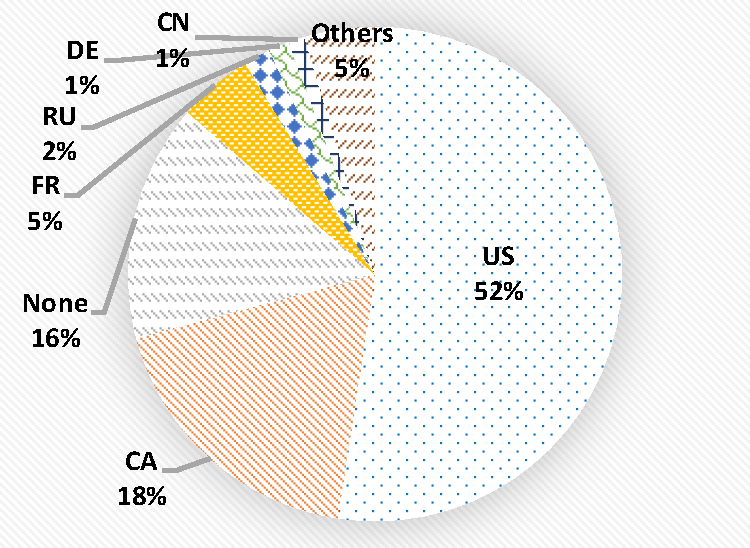
\includegraphics[width=2in]{figure/countryPie}
\caption{How PE submissions distribute among different countries.
%\footnotesize{
(Only countries with more than 1\% PE submissions are shown.)
%}
}
\label{fig:countryPie}
\end{center}
%\vspace{-0.25in}
\end{figure}

For around 16\% of PE submission, 
\vt\ fails to provide their source country information. 
All other submissions are conducted from 221 countries. 
The top 6 countries in PE submission number are US, Canada, France, Russia, Germany, and China, 
as shown in Figure~\ref{fig:countryPie}.

\begin{figure}[t!]
\begin{center}
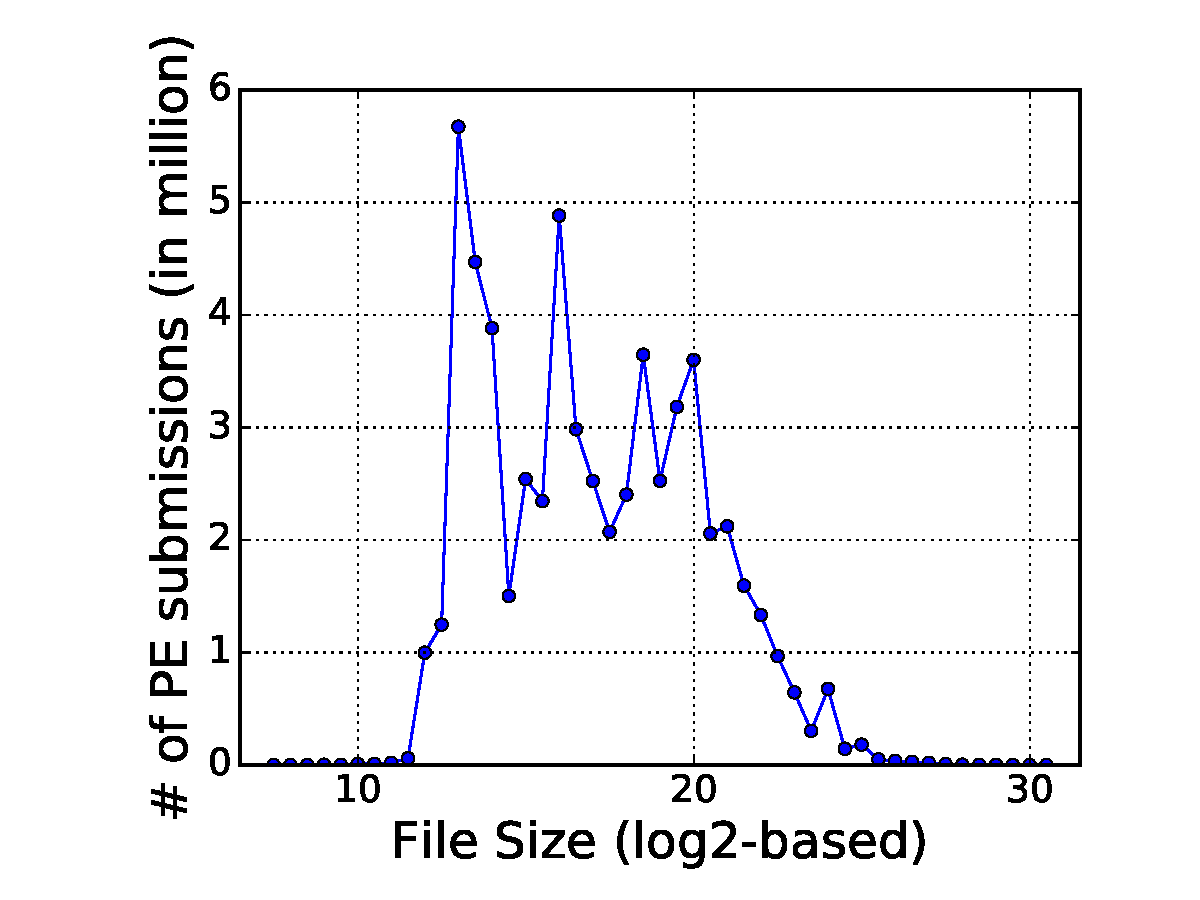
\includegraphics[width=2.5in]{figure/pesize}
\mycaption{fig:pesize}{File size distribution for PE submissions.}
{\footnotesize{(How file size distributes among all PE submissions we collect. 
Results from log2 are rounded up to nearest 0.5.)}}
\end{center}
%\vspace{-0.25in}
\end{figure}

Figure~\ref{fig:pesize} shows the file size distribution for \pe\ submissions. 
The smallest \pe\ file is only 187 bytes, and the largest one is more than 1\,GB. 
99.58\% of PE file fall into the range from 4\,KB to 32\,MB. 

{\bf Observation 1:} 
{\em \vt\ constantly receives large amount of submissions from all over the world. 
Most submitted files have small to middle sizes and are only submitted once, 
but some files are submitted many times.}

%\noindent{\textit{\underline{Submission sources.}}}
\subsection{Source ID}
\label{sec:source_id}

\begin{figure}[t!]
\begin{center}
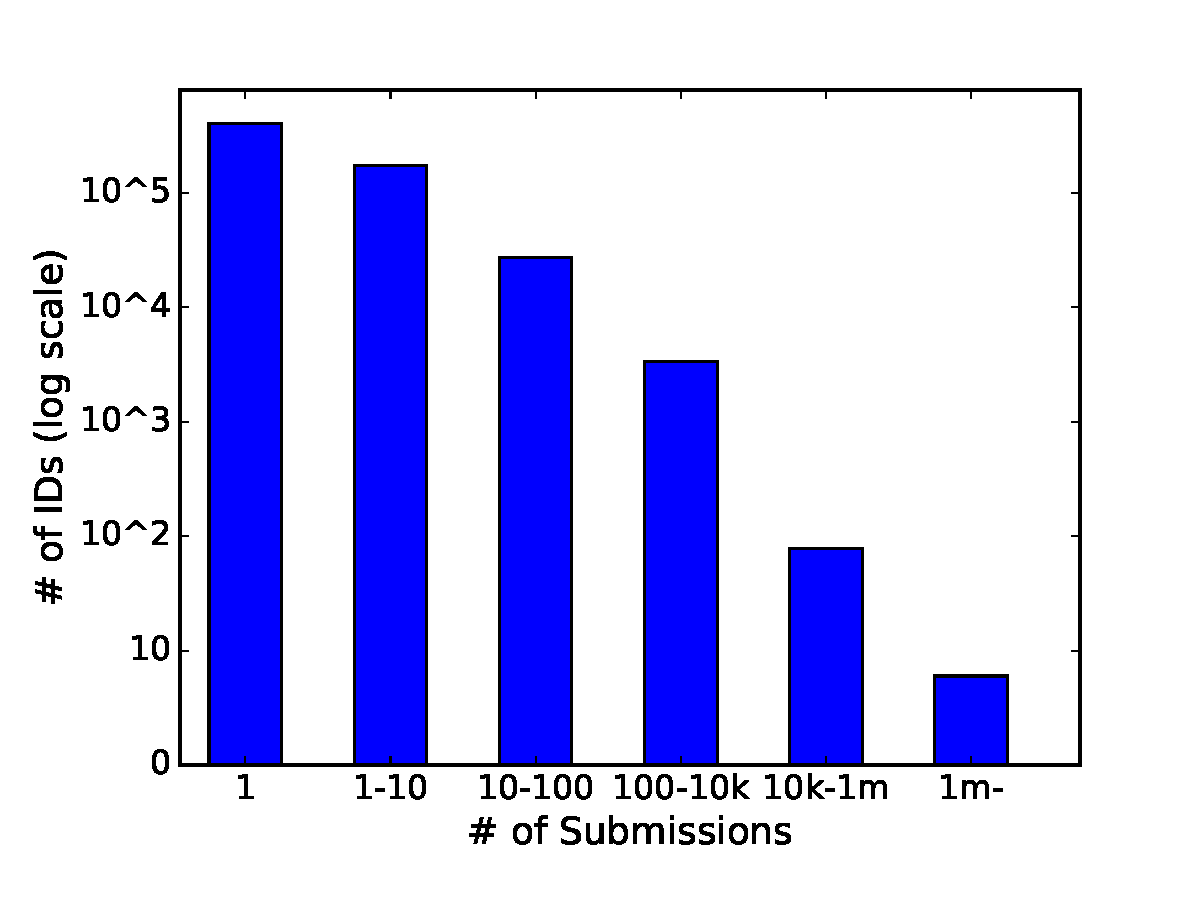
\includegraphics[width=2.5in]{figure/IDDistribution}
\mycaption{fig:iddis}{The distribution for source ids.}
{\footnotesize{(How source ids distribute among all source id groups. 
We divide groups based on PE submissions made by each source id.)}}
\end{center}
%\vspace{-0.25in}
\end{figure}

Both normal users and anti-virus vendors use \vt\ to detect malwares or evaluate products.
Usually, vendors tend to make more submissions than normal users, since they need to test their products on many files.
Thus, we use the number of submissions to measure what type of users a source ID is.

We separate the number of submissions into six categories:
one submission, one to ten submissions, ten to 100 submissions, 100 to 10000 submissions, 10000 to 1 million submissions, and larger than 1 million submissions.
Figure~\ref{fig:iddis} plots the number of source IDs in log scale in the first five categories.
There are only 6 source IDs that have more than 1 million submissions and we suspect that these IDs are either bogus or robots 
that constantly make submissions to \vt.
For the rest, we find that the number of source IDs dramatically drops when the number of submissions is more than 100.
Thus, we categorize the source IDs as normal user if they have less than 100 submissions and as vendors if they have more than 100 submissions.

{\bf Observation 2:} 
{\em Most \vt\ users are normal users that make occasional submissions, while a small set of anti-virus vendors use \vt\ and make a huge amount of submissions.}


%\noindent{\textit{\underline{Anti-virus engines and detection basic analysis.}}}

\subsection{Anti-virus Engines}

\begin{figure}[t!]
\begin{center}
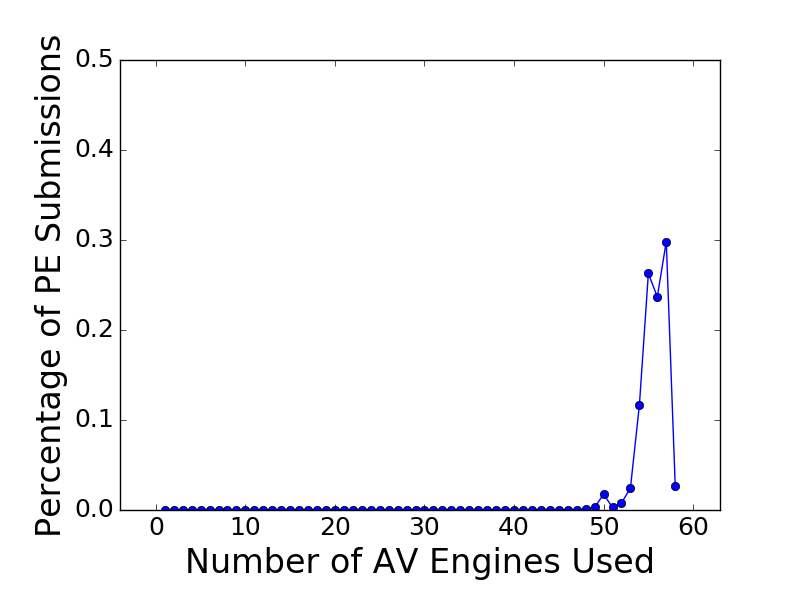
\includegraphics[width=2in]{figure/numVendor}
\caption{The distribution for the number of used anti-virus engines.
(How the number of applied anti-virus engines distributes among all PE submissions.
)
}
\label{fig:vendornum}

\end{center}
%\vspace{-0.25in}
\end{figure}
\begin{figure}[t!]
\begin{center}
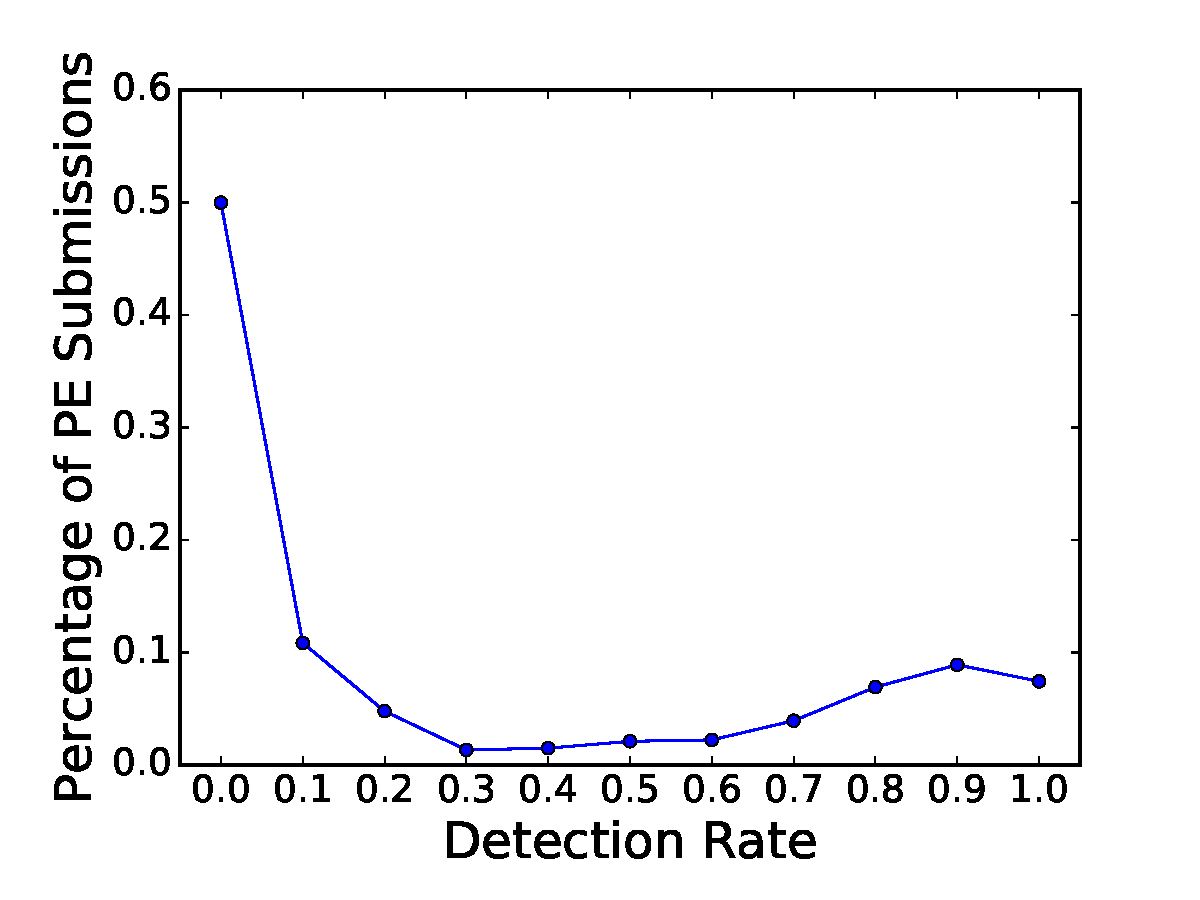
\includegraphics[width=2in]{figure/DetectionRate}
\caption{The distribution for detection rate.
(How detection rate distributes among all PE submissions. 
Each detection rate is rounded up to nearest 0.05.)
}
\label{fig:detectiorate}
\end{center}
%\vspace{-0.25in}
\end{figure}


After learning the basic properties of submissions and source IDs, 
we now move to the basic analysis of anti-virus engines and their detection of malware.
Figure~\ref{fig:vendornum} shows the distribution of the number of anti-virus engines used by \vt\ on each submission. 
More than 99\% of PE submissions are analyzed by at least 50 anti-virus engines. 
We suspect that \vt\ sets some threshold when running anti-virus engines and 
will abort an engine when it takes too long to run on a submission,
causing few submissions having fewer than 50 engines.

For the same submission, different anti-virus engines can make different detection results, \ie, 
some mark the submission as malware while others don't.
To quantify the detection results of a submission,
we use a value we call {\em Detection Rate}.
Detection rate represents the percentage of engines labeling the submission as malware. 

$$ \textrm{\textit{Detection Rate}} = \dfrac{positives}{total + 1}$$

We add one to {\bf total} to avoid divide-by-zero exception, and more importantly, 
to have higher detection rate to submissions labeled as malwares by more engines.
For example, submissions analyzed by 50 engines and detected by 50 engines 
has a higher detection rate 
than submissions analyzed by one engine and detected by one engine. 
%This formula shares the same intuition from previous work~\cite{GuoICSE2010}, when computing reputations for bug reporters. 
%A larger detection rate usually indicates a more malicious malware suggested by analyzed anti-virus engines. 

Figure~\ref{fig:detectiorate} shows the distribution of detection rates over all \pe\ submissions.
We separately consider submissions made by normal users and by anti-virus vendors 
(as defined in Section~\ref{sec:source_id}).
Interestingly, overall most submissions to \vt\ are likely to be benign files, \ie, has low detection rate.
Around half of the submissions were labeled as benign by all engines (a detection rate of zero),
and only 31.5\% submissions were labeled as malware by at least half of the engines.
Surprisingly, the detection rates of submissions made by normal user and by anti-virus vendors are very similar.
One probable explanation is that anti-virus vendors obtain their suspicious files 
from end users and thus have similar behavior as normal users' submissions.
Another possible reason is that as suspicious files are announced publicly, 
both normal users and vendors will try to test them with \vt.



{\bf Observation 3:} 
{\em Most submissions to \vt\ are labeled as benign and 
submissions made by normal user and by anti-virus vendors have similar probabilities of being labeled as malware.}


